\chapter{L'entreprise et la bourse}

\section{Nature et forme des entreprises}

\begin{itemize}
    \item \textblue{SLR} - Société à Responsabilité Limitée
    \item \textblue{SA} - Société Anonyme
    \item \textblue{SC} - Société Coopérative
\end{itemize}

\section{Séparation propriété-gestion}

\begin{itemize}
    \item Dans une SA, la propriété et le contrôle sont distincts
    \item Assemblée générale des actionnaires
    \begin{itemize}
        \item Approuve les comptes annuels et la politique de rémunération des actionnaires
        \item Désigne les administrateurs
        \item Donne d"charge aux administrateurs et réviseurs
    \end{itemize}
    \item Le conseil d'administration
    \begin{itemize}
        \item Désigne un (ou plusieurs) administrateurs délégués à la gestion journalière, généralement le CEO
    \end{itemize}
    \item Chief Financial Officer (CFO)
    \begin{itemize}
        \item Gère les décisions d'investissement, financement et pour la trésorerie
    \end{itemize}
\end{itemize}

\section{Regard critique}

Le management prend des décisions afin de maximiser la valeur de l'entreprise
\begin{itemize}
    \item Sans porter préjudice à l'ensemble des stakeholders
    \item Dans le respect de l'éthique et de l'environnement
    \item Volonté d'impact sur la société et l’environnement (SDG - Sustainable Development Goods)
    \item[$\rightarrow$] Corporate Sustainability Reporting Directive (CSRD)
\end{itemize}

\section{Les marchés boursiers}

\begin{itemize}
    \item \textblue{Marchés primaires} : ex. Lorsque l'entreprise lève des fonds
    \item \textblue{Marchés secondaires} : Une fois les titres émis sur le marché primaire, ils sont négociés sur le marché secondaire
    \item \textblue{Actions} :
    \begin{itemize}
        \item Participation au capital d'une entreprise
        \item Potentiel élevé de rendement, mais avec des fluctuations importantes $\rightarrow$ risque plus élevé
    \end{itemize}
    \item \textblue{Obligations} :
    \begin{itemize}
        \item Prêt à une entité avec engagements de remboursement avec intérêts
        \item Moins risqué que les actions, mais dépend de la quantité de crédit de l'émetteur
        \item Payements d'intérêts réguliers (coupons)
    \end{itemize}
    \item \textblue{Cash} : 
    \begin{itemize}
        \item Comptes épargnes, dépôts à vue
        \item Risque très faible, mais rendement nul
    \end{itemize}
\end{itemize}

\addtocounter{chapter}{1}
\chapter{Arbitrage et décisions financières}

\section{Décisions financières}

Basées uniquement sur des valeurs actualisées (VA)

\section{Taux d'intérêt et valeur temporelle de l'argent}

Exemple : nous investissons de 100€ à 5\% sur 1 an :
\begin{itemize}
    \item 100€ correspond à la valeur actuelle (VA)
    \item 5\% correspond au taux d'actualisation de taux sans risque (E(R))
    \item la valeur future (VF)  est égale à $100 + 100 * 0.05 = 105$€
\end{itemize}

\begin{itemize}
    \item[$\hookrightarrow$] \textblue{Return} $= 5\% = \frac{105-100}{100} \rightarrow 100 = \frac{105}{1 + 0.05}$
    \item[$\hookrightarrow$] \textblue{$VA$} $= \frac{VF}{1 + E(R)} \leftrightarrow \textblue{VF} = VA * (1 + E(R))$
\end{itemize}

\section{La valeur actuelle et la règle de décision VAN}

\begin{itemize}
    \item \textblue{Valeur Actuelle Nette} (VAN) = valeur actuelle des recettes (cash flow > 0) - valeur actuelle de ses coûts (cash flow < 0)
    \item \textblue{Règle de décision} :
    \begin{itemize}
        \item[\textgreen{V}] si VAN $\geq 0 \rightarrow$ favorable de maximiser la VAN
        \item[\textred{X}] si VAN $< 0$
        \item Si toutes les options d'investissement sont à un an et sans risque $\rightarrow$ taux d'actualisation = 2\%
    \end{itemize}
\end{itemize}

\section{Arbitrage et la loi de prix unique}

\begin{itemize}
    \item \textblue{Arbitrage} :
    \begin{itemize}
        \item Achat-revente de biens équivalents sur des marchés différents pour profiter d'une différence de prix
        \item Possibilité de réaliser un profit sans prendre de risque ni faire d'investissements
    \end{itemize}
    \item \textblue{Marché normal} : marché concurrentiel sans opportunités d'arbitrage
    \item \textblue{Loi du prix unique} : si des opportunités d'investissement se présentent sur différents marchés concurrentiels, elles doivent se négocier au même prix
\end{itemize}

\section{Absence d'arbitrage et valeurs des titres}

Si le prix = $940$€ :
\begin{itemize}
    \item[$\rightarrow$] Achat de l'obligation et emprunt à 1 an de $1000$€ à 5\%
    \item Cash de l'emprunt : $VA = \frac{100}{1.05} = 952.4$€ $\rightarrow$ on reçoit ajd $952.4$€
    \item Cash de l'achat de l'obligation : $-940$€
    \item Solde : $952.4 - 940 = 12.4$€ $\rightarrow$ cash directement en poche
\end{itemize}
Dans 1 an :
\begin{itemize}
    \item Remboursement du prêt : $-1000$€
    \item Récupération de la valeur de l'obligation : $+1000$€
    %\item Total : $0$€
\end{itemize}

\chapter{La valeur temps de l'argent}

\section{L'échéance}

ou diagramme des flux :
\begin{figure}[H]
    \centering
    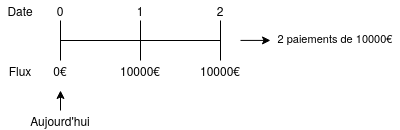
\includegraphics[width=0.57\textwidth,keepaspectratio]{flux}
\end{figure}

\section{Actualisation - Capitalisation}

\begin{itemize}
    \item[$\rightarrow$] Permet de comparer des sommes disponibles à des dates différentes
    \item \textblue{Capitalisation} : présent $\rightarrow$ avenir
    \item \textblue{Actualisation} : présent $\leftarrow$ avenir
    \item Capitalisation - intérêts composés :
    \begin{itemize}
        \item[$\rightarrow$] La VF d'un placement en $0$ pour $t$ périodes au taux d'intérêt composé $i$ est égal à :
        \begin{align*}
            &VF(A@i\%) = A * (1 + i)^t &&&&& (t > 1 \text{ an})
        \end{align*}
    \end{itemize}
    \begin{itemize}
        \item[$\rightarrow$] Si intérêt simple :
        \begin{align*}
            &VF(A@i\%) = A * (1 + i * t) & (t < 1 \text{ an, ex : 3 mois}\rightarrow t = 0.25)
        \end{align*}
    \end{itemize}
    \item Ex : on propose un investissement donnant un cash flow de 121€ dans 2 ans. On attend un return de 10\%. Combien investit-on ? $VA = \frac{121}{(1 + 0.1)^2} = 100$€
    \item[$\rightarrow$] Valeur actuelle d'un cash flow A : $VA (A@i\%) = \frac{A}{(1 + I)^t}$
\end{itemize}

\section{Valeur actuelle et future d'une séquence de flux}

\begin{align*}
    VF &= A * \left[ \frac{(1 + i)^n - 1}{i}         \right] \\
    VA &= A * \left[ \frac{1 - 1/(1+i)^n}{i} \right]
\end{align*}

Ex : Quel montant $x$ faut-il épargner annuellement au cours des $20$ prochaines années afin de percevoir une rente annuelle de $10000$€ pour les 20 prochaines années qui suivent ? Le taux d'intérêt est de 5\%.
\begin{itemize}
    \item[$\rightarrow$] La valeur future de $x$ à l'année 20 doit être égale à la valeur actuelle de $A$ à l'année $20$ :
\end{itemize}
\begin{align*}
    x * \left( \frac{(1 + 0.05)^{20} - 1}{0.05} \right) &= 10000 * \left( \frac{1 - 1/(1 + 0.05)^{20}}{0.05} \right) \\
    \Leftrightarrow x &= 3.769
\end{align*}

\section{Rentes perpétuelles, annuités et autres cas particuliers}

\begin{itemize}
    \item Valeur actuelle au taux $i$ d'un cash flow constant $A$ :
    \begin{align*}
        VA = \frac{A}{i}
    \end{align*}
    \item Valeur actuelle au taux $i$ d'i, cash flow $A$ de croissance constante $g < i$ :
    \begin{align*}
        VA = \frac{A_1}{i - g} && A_t = A_1 * (1 + g) t - 1
    \end{align*}
\end{itemize}

\section{Valeur actuelle nette d'une séquence de flux}

VAN = valeur actuelle de tous les cash flows d'un projet :
\begin{align*}
    VAN = \sum_{t = 0}^T \frac{CF_t}{(1 + E(R))^t}
\end{align*}

\section{Flux infra-annuels}

\warning Cohérence des unités : les périodes et le taux d'actualisation doivent être exprimés dans les mêmes unités (ex : périodes annuelles et taux annuel ou périodes mensuelles et taux mensuels)

\section{Calculer les montants à payer, le TRI, le nombre de périodes}

\begin{itemize}
    \item \textblue{TAEG} : Taux Annuel Effectif Global
    \item \textblue{TRI} : Taux de Rentabilité Interne
    \begin{itemize}
        \item[$\rightarrow$] Taux d'actualisation des cash flows t.q. $VAN = 0$
        \item[$\rightarrow$] $VAN = 0 = \sum_{t = 0}^T \frac{CF_t}{(1 + TRI)^t}$
        \item Correspond à la rentabilité attendue d'un projet
    \end{itemize}
\end{itemize}

\textblue{Note} : lorsqu'il s'agit d'un financement (CF > 0 suivi de paiements) TRI = coût d’emprunt)

\addtocounter{chapter}{1}
\chapter{La valorisation des obligations}

\textblue{Définition} : titre obligeant l'émetteur à effectuer des paiements déterminés au détenteur de l'obligation.

\section{Caractéristiques des obligations}

\begin{itemize}
    \item \textblue{Émetteur}
    \begin{itemize}
        \item Gouvernement
        \item Corporate : Junior (obligations remboursées après Senior, Risque $\nearrow$ : taux d'intérêt $\nearrow$) vs Senior (remboursés en premier)
    \end{itemize}
    \item \textblue{Fréquence de coupon} : paiements des intérêts aux obligataires
    \item \textblue{Taux de coupon}
    \item \textblue{Valeur nominale} : Généralement remboursée à la maturité
    \item \textblue{Cotation} :
    \begin{itemize}
        \item Un pourcentage de la valeur nominale
        \item Intérêt connu
    \end{itemize}
    \item \textblue{Rating} : de AAA (très safe) à C (pas safe du tout ; prime de risque $\nearrow$ (spread))
    \begin{itemize}
        \item[$\rightarrow$] \textblue{Taux de défaut} : probabilité que l'émetteur de l'obligation ne puisse pas honorer ses paiements d'intérêts ou rembourser le capital à l'échéance
        %\item \textblue{Note} : plus le spread $\nearrow$ plus le taux de défaut $\nearrow$
    \end{itemize}
    \item \textblue{Corporate bonds} : titres de créances émis par des entreprises pour lever des fonds
    \begin{itemize}
        \item Classement : Haute qualité (> BBB) $\rightarrow$ Haute performance (BB <)
    \end{itemize}
    \item Dirty price = clean price + intérêt couru
    \item[$\hookrightarrow$] intérêt couru = coupon annuel $* \frac{\text{\# jours écoulés}}{\text{\# jours entre 2 paiements}}$
\end{itemize}

\section{Prix et yields}

\begin{itemize}
    \item \textblue{Prix des obligations} (PV) : valeur actuelle des flux de trésorerie future
    \begin{align*}
        PV &= \sum_{t = 1}^T \frac{CF_t}{(1+E[R])^t}\\
           &= \sum_{t=1}^T \frac{C}{(1+E[R])^t} + \frac{R}{(1 + E[R])^T}\\
           &= C * \left[ \frac{1 - 1/(1+E[R])^T}{E[R]} \right] + \frac{R}{(1 + E[R])^T}
    \end{align*}
    Où :
    \begin{itemize}
        \item $C$ = paiement périodique du coupon
        \item $R$ = remboursement final (souvent égal à la valeur nominale)
        \item $E[R]$ = rendement
    \end{itemize}
    \item Si le taux d'intérêt du marché est supérieur (inférieur) au taux du coupon, les obligations se vendent à un prix inférieur (supérieur) à leur valeur nominale
    \item \textblue{Current yield} = coupon annualisé divisé par le prix
    \item \textblue{Yield to Maturity} (YTM) = taux d'actualisation (return attendu) pour lequel la valeur actuelle des flux futurs est égal au prix (dirty price) actuel
    \item \textblue{Premium bond} (prix > valeur nominale) : Current Yield > YTM
    \item \textblue{Discount bond} (prix < valeur nominale) : Current Yield < YTM
    \item \textblue{Rate of return} : revenu total (coupon + variations de prix) par période et euro investi
    \item[$\hookrightarrow$] $R = \frac{P_1 - P_0}{P_0} + \frac{C}{P_0}$
    \begin{itemize}
        \item[$=$] YTM si intérêt stable et l'obligation est conservée jusqu'à échéance
    \end{itemize}
\end{itemize}

\subsection{Current Yield VS YTM}

\begin{itemize}
    \item \textblue{Current yield} : 1er indicateur du rendement d'une obligation, mais pas précis car il ne prend pas en compte la génération de gais ou pertes
    \item \textblue{YTM} mesure plus précise, prend en compte les flux de trésorerie et l'écart entre le prix d'achat actuel et la valeur de remboursement de l'obligation à échéance
\end{itemize}

\section{Risque de taux}

\begin{itemize}
    \item Les obligations à long-terme sont plus sensibles aux variations des taux d'intérêt que celles à court-terme
    \begin{itemize}
        \item[$\rightarrow$] si le taux d'intérêt $\nearrow$, plus l'obligation est longue, plus la perte d'opportunité grandie
    \end{itemize}
    \item \textblue{Volatilité des obligations} : diminue (augmente) si le rendement augmente (diminue)
    \item \textblue{Risque de taux d'intérêt} : le détenteur de l'obligation décide de la vendre avant son échéance (souvent car le taux d'intérêt augmente)
    \item \textblue{Duration} (D) : évalue la sensibilité du prix d'une obligation à une variation des taux d'intérêt :
    \begin{align*}
        D &= \sum_{t=1}^T w_t * t \text{, avec } w_t = \frac{CF_t}{(1+YTM)^t} / \sum_{k=1}^T \frac{CF_k}{(1 + YTM)^k}
    \end{align*}
\end{itemize}

\section{Arbitrage : Taux variable vs Taux fixe à long terme}

\begin{itemize}
    \item Taux variable (taux de référence + spread)
    \begin{itemize}
        \item Financement à un taux plus faible
        \item Risque sur la charge d'intérêt
        \item La prime de risque (spread) est fixe
    \end{itemize}
    \item Taux fixe
    \begin{itemize}
        \item Taux plus élevé
        \item Pas de risque sur la charge d'intérêt
    \end{itemize}
\end{itemize}

\section{Prime de risque (spread)}

\begin{itemize}
    \item[$=$] différence de rendement entre une obligation du Trésor équivalente et une obligation d'entreprise
    \item Fonction de :
    \begin{itemize}
        \item Probabilité de défaut ($\lambda$)
        \item Taux de recouvrement ($R$)
        \item Prix du risque sur le marché ($r$)
    \end{itemize}
    \item[$\rightarrow$] Spread = $\lambda (r - R)$, où $\lambda$ est la probabilité de défaut, et $R$ le taux de recouvrement
\end{itemize}

\chapter{Règles de décision et d'investissement}

\section{La valeur actuelle nette}

\begin{itemize}
    \item[$=$] valeur actuelle de tous les cash flows
    \begin{align*}
        VAN = \sum_{t=0}^T \frac{CF_t}{(1 + E[R])^t}
    \end{align*}
    \item[$\hookrightarrow$] si $VAN > 0$ :
    \begin{itemize}
        \item VA des investissements < VA des cash flows générés par l'investissement
        \item valeur de l'entreprise $\nearrow$
        \item l'entreprise va réussir à récupérer le capital investi, rémunérer les bonds immobilisés selon les exigences des investisseurs, dégager du surplus pour les actionnaires dont la VA est égale à la VAN du projet
    \end{itemize}
    \item taux d'actualisation = coût d'opportunité du capital, c.-à-d. la rentabilité à laquelle les investisseurs renoncent pour entreprendre le projet
    \item risque intégré via le taux de rentabilité attendu
\end{itemize}

\section{Taux de rentabilité interne}

\begin{itemize}
    \item \textblue{Hypothèse de réinvestissement} : Pour que la rentabilité d’un investissement soit égale au TRI, il est indispensable que l’investissement soit maintenu jusqu’à la date de fin et que tous les cash flows intermédiaires soient réinvestis dans des projets de rentabilité égale au TRI
    \item \textblue{Critère de décision} : tout projet dont TRI > coût d'opportunité du capital devrait être accepté
    \item Critère de VAN préférable car en ligne avec l'objectif de maximisation de la valeur et ne fait pas l'hypothèse de réinvestissement (contrairement au TRI)
\end{itemize}

\section{Délai de récupération (payback)}

\begin{itemize}
    \item[$=$] temps nécessaire pour que les cash flows remboursent l'investissement initial
    \begin{align*}
        \sum_{t=1}^{payback} CF_t - I_0 \geq 0
    \end{align*}
    \warning Ne tient pas compte de tous les cash flows réalisés après le payback
    \item[$\rightarrow$] \textblue{Délai de récupération actualisé (Discount payback)} = temps nécessaire pour que la VAN des cash flows cumulés actualisés devienne > 0
    \begin{align*}
        \sum_{t=1}^{payback} \frac{CF_t}{(1 + E[R])^t} - I_0 \geq 0
    \end{align*}
\end{itemize}

\section{L'indice de probabilité}

\begin{itemize}
    \item Mesure la VAN en \% des capitaux investis
    \item Mesure l'efficacité de l'utilisation des ressources
    \begin{align*}
        IP = \frac{VAN}{\sum_{t=0}^T \frac{I_t}{(1+E[R])^t}}
    \end{align*}
\end{itemize}

\chapter{Éléments de la décision d'investissement}

\section{Résultats attendus}

\begin{itemize}
    \item \textblue{Résultats d'exploitation}
    \begin{center}
    \begin{tabular}{|c|l|l|}
    \hline 
    \textgreen{+} & Ventes &  \\ 
    \hline 
    \textred{-} & Coût des unités vendues &  \\ 
    \hline 
    $\hookrightarrow$ & = & \textblue{Gross Profit} \\ 
    \hline 
    \textred{-} & Frais de vente, marketing, administratif & \\ 
    \hline 
    \textred{-} & Frais de R\&D &  \\ 
    \hline 
    \textred{-} & Amortissement &  \\ 
    \hline 
    $\hookrightarrow$ & = & \textblue{Ernings Before Interest and Taxes (EBIT)} \\ 
    \hline 
    \textred{-} & Impôts &  \\ 
    \hline 
    = & \textblue{Résultat net d'exploitation} &  \\ 
    \hline 
    \end{tabular}
    \end{center}
    \item \textblue{Résultats incrémentaux} : comparaison des composantes avec et sans investissement
    \item \textblue{Sunk cost} : cash flows engagés et non récupérables
    \item \textblue{Règle} : si la décision d'investir n'a aucun impact sur un cash flow, alors ce cash flow n'est pas pris en compte dans la décision d'investir
\end{itemize}

\section{Free cash flow et calcul de la VAN}

\begin{itemize}
    \item \textblue{Résultats d'exploitation}
    \begin{center}
    \begin{tabular}{|c|l|}
    \hline 
    \textgreen{+} & Amortissement \\
    \hline 
    \textred{-} & CAPEX \\
    \hline
    \textred{-} & Augmentation BFR \\
    \hline 
    \textgreen{+}/\textred{-} & Cash flows de fin \\
    \hline
    = & \textblue{Free cash flows} \\ 
    \hline 
    \end{tabular}
    \end{center}
    \begin{itemize}
        \item[$\hookrightarrow$] permet d'analyser un projet d'investissement
    \end{itemize}
    \item VAN = $\sum_{t=0}^T \frac{\text{Flux de trésorerie disponible}}{(1+\text{opportunité du capital})^t}$
\end{itemize}

\section{Choix entre des projets}

\begin{itemize}
    \item[$\rightarrow$] Choix de la VAN la + élevé
    \item[\warning] Cas particuliers : projet de remplacement de choix entre différents équipements
    \begin{itemize}
        \item[$\hookrightarrow$] calcul du coût annuel équivalent (CAE)
        \begin{align*}
            VAN = \sum_{t=0}^T \frac{FCF_t}{(1 + E[R])^t} = CAE * \frac{1 - \left(\frac{1}{1 + E[R]} \right)^T}{E[R]}
        \end{align*}
        \item Si frais sur 1 an max : VAN = CAE
    \end{itemize}
\end{itemize}

\chapter{Valorisation des actions}

\begin{itemize}
    \item \textblue{Action} :
    \begin{itemize}
        \item Droit de propriété
        \item Droit aux dividendes
        \item Droit de vote / gestion
        \item[$\rightarrow$] Pour financer des investissements, les entreprises lèvent des capitaux par émissions d'actions
    \end{itemize}
    \item \textblue{Earning Per Share (EPS)} : résultat par action
    \item \textblue{Price Earning Ratio (PER ou P/E)} : utilisé pour évaluer la valorisation d'une entreprise
    \begin{itemize}
        \item[$=$] $\frac{\text{Prix de l'action}}{\text{Résultat par action (EPS)}}$
        \item[$\rightarrow$] Si élevé : peut indiquer que les investisseurs s'attendent à une forte croissance future des bénéfices de l'entreprise. Cependant, peut-être que l'action est surévaluée
        \item[$\rightarrow$] Si faible : action sous-évaluée ou entreprise avec des difficultés financières
    \end{itemize}
    \item \textblue{Rendement de l'action / dividend yield}
    \begin{itemize}
        \item[$=$] $\frac{\text{Dividende annuelle par action}}{\text{Prix de l'action}}$
        \item[$\rightarrow$] Si élevé : l'entreprise reverse une par importante de ses bénéfices sous forme de dividendes (attractif pour revenus réguliers) mais peut aussi indiquer un prix d'action bas et des problèmes financiers potentiels
        \item[$\rightarrow$] Si faible : l'entreprise réinvestit une grande partie de ses bénéfices dans la croissance future (attractif car croissance LT)
    \end{itemize}
    \item \textblue{Valeur comptable} (état financier) : application de règles pour enregistrer la valeur des actifs et leur financement
    \item \textblue{Valeur de liquidation} (vente rapide) : montant espéré de la vente des actifs après remboursement de toutes les dettes
    \item \textblue{Valeur de marché} (offre / demande) : valeur économique qui prend en compte :
    \begin{itemize}
        \item les opportunités d'investissement futur
        \item les actifs intangibles t.q. l’organisation, la marque, etc
        \item la capacité des actifs à générer plus de valeur en étant dans l'entreprise (extra earning power)
    \end{itemize}
\end{itemize}

\section{Dividend Discount Model}

\begin{itemize}
    \item \textblue{Prix de l'action} $=$ $P_0 = \frac{D_1 + P_1}{1 + E[R]}$, où :
    \begin{itemize}
        \item $D_1$ = dividende attendu
        \item $P_1$ = prix de vente de l'action
        \item $E[R]$ = rentabilité de l'actionnaire
    \end{itemize}
    \item[$\rightarrow$] la rentabilité attendue inclut un taux de dividende (dividend yield) et une plus-value (capital gain) :
    \begin{itemize}
        \item $E[R] = \frac{D_1}{P_0} + \frac{P_1 - P_0}{P_0}$, où :
        \begin{itemize}
            \item $\frac{D_1}{P_0}$ = dividend yield
            \item $\frac{P_1 - P_0}{P_0}$ = capital gain
        \end{itemize}
    \end{itemize}
    \item Si multipériodique $P_0 = \sum_{t=1}^N \frac{D_t}{(1 + E[R])^t} + \frac{P_N}{(1 + E[R])^N}$
    \item \textblue{Dividende constant} :
    \begin{align*}
       P_0 = \sum_{t=0}^{\infty} \frac{D}{(1 + E[R])^t} &\xrightarrow{\infty} P_0 = \frac{D}{E[R]} \\
         &\hookrightarrow P_0 = \frac{EPS * (1-b)}{E[R]} = EPS * \frac{1-b}{E[R]}
    \end{align*}
    $\rightarrow$ Prix de l'action = multiple des résultats
    \item \textblue{Croissance constante} : on vérifie que la croissance $g$ du dividende est $g = b * ROE$ (ROE = $\frac{\text{Bénéfices net}}{\text{Capitaux propres}}$)
    \item Dès lors :
    \begin{align*}
        D_t &= D_{t-1} * (1 + g) &&&&&&&&&&\\
        D_t &= D_1 * (1+g)^{t-1} &&&&&&&&&&
    \end{align*}
    \item Le DDM devient :
    \begin{align*}
        P_0 &= \sum^{\infty}_{t=1} \frac{D_1 * (1+g)^{t-1}}{(1+E[R])^t} = \frac{D_1}{E[R] - g} &&&&&&&&
    \end{align*}
    \item[$\hookrightarrow$] aussi appelé le modèle de Gordon et Shapiro
    \begin{align*}
        P_0 &= \frac{D_1}{E[R] - g} & E[R] = \frac{D_1}{P_0} + g &&&&&&&&
    \end{align*}
\end{itemize}

\section{Modèle des Free Cash Flows}

\begin{itemize}
    \item Valeur d'une entreprise (EV) :
    \begin{align*}
        EV = \sum_{t=1}^{\infty} \frac{FCF_t}{(1 + WACC)^t}
    \end{align*}
    \item $FCF_t$ est le Free Cash Flow attendu en $t$
    \begin{align*}
        FCF_t = EBIT_t * (1-r) &+ \text{Amortissement} \\
                               &- \text{Investissement} \\
                               &- \text{Augmentation du BFR}
    \end{align*}
    \item $WACC$ = coût moyen pondéré du capital
    \begin{align*}
        WACC = \frac{E}{E+D} * E[R_R] + \frac{D}{E+D} * E[R_D] * (1-\tau)
    \end{align*}
    \item Valeur de marché des fonds propres (MVE)
    \begin{align*}
        MVE = EV - Debt + cash
    \end{align*}
\end{itemize}
\begin{align*}
    &\Longrightarrow EV = \frac{FCF_1}{(1 + WACC)} \cdot \cdot \cdot \frac{FCF_5}{(1 + WACC)^5} + \frac{TV_5}{(1 + WACC)^5}\\
    &\text{Où } TV_5 = \frac{FCF_5 * (1-g)}{WACC - g}
\end{align*}

\subsection{Valorisation par la méthode des comparables}

Technique de valorisation utilisée pour estimer la valeur d'une entreprise en comparant ses ratios financiers à ceux d'entreprises similaires. Le choix des entreprises comparables se fait sur des critères t.q. :
\begin{itemize}
    \item Stade de développement / croissance attendue
    \item Business Model
    \item Taille et localisation du marché cible
    \item Taille de l'entreprise
    \item Niveau de risque
    \item ...
\end{itemize}

\newpage
\subsection{Information et efficience du marché}

Hypothèse de l'efficience des marchés :
\begin{itemize}
    \item Les prix des tires reflètent rapidement les nouvelles informations, qui arrivent de manière aléatoire
    \item Les prix semblent suivent un marché aléatoire
    \item 3 types d'information et 3 degrés d'efficience :
    \begin{itemize}
        \item \textblue{Forme faible}
        \begin{itemize}
            \item Prix reflètent toute l'information contenue dans les prix passés
            \item Variations de prix aléatoires
            \item Analyse technique sans valeur
        \end{itemize}
        \item \textblue{Forme semi-forte}
        \begin{itemize}
            \item Prix reflètent toute l'information contenue dans les prix passés et toute l'information disponible publiquement
            \item Impossible d'obtenir des rendements constamment supérieurs
        \end{itemize}
        \item \textblue{Forme forte}
        \begin{itemize}
            \item Prix reflètent toute l'information disponible, publique et privée
            \item Impossible d'obtenir un rendement supérieur constant
        \end{itemize}
    \end{itemize}
\end{itemize}

\chapter{Marché financier et prime de risque}

\section{Risque et return}

\begin{itemize}
    \item Return attendu : $E[R_{ptf}] = R_f + Prime$
    \item Risque = exposition à l'incertitude
    \item Plusieurs sources d'incertitude :
    \begin{itemize}
        \item \textblue{Évolution des marchés} (prix, taux de change, taux d'intérêt, défaut sur la dette, etc)
        \item Opérationnel (systèmes, procédures, facteur humain)
        \item Réputation
        \item Risque de transition / climatique
        \item Autres
    \end{itemize}
    \item Mesure du risque = Écart-type des returns
\end{itemize}

\section{Rappel statistique}

\begin{itemize}
    \item Moyenne des returns
    \begin{align*}
        \bar{R}_i = \sum_{j=1}^N \frac{R_{ij}}{N}
    \end{align*}
    \item Écart-type : dispersion des retours de l'actif i autour de sa moyenne
    \begin{align*}
        \sigma (R_i) = \sqrt{\sum_{j=1}^N \frac{(R_{ij} - \bar{R}_i)^2}{N - 1}}
    \end{align*}
    \item Covariance : comment le retour des 2 actifs varient ($> 0$ : même direction, $< 0$ : sens opposé)
    \begin{align*}
        \sigma (R_i, R_j) = \sigma_{ij} = \sum_{k=1}^N \frac{(R_{jk} - \bar{R}_i)(R_{jk} - \bar{R}_j)}{N - 1}
    \end{align*}
    \item Corrélation : 1 = relation positive, 0 = absence de relation linéaire, -1 : relation négative
    \begin{align*}
        \rho_{ij} = \frac{\sigma(R_i, R_j)}{\sigma(R_i)\sigma(R_j)}
    \end{align*}
    \item Espérance du return : $w_i$ = poids de l'actif $i$ dans le portefeuille
    \begin{align*}
        E[R_{ptf} = \sum_{i=1}^N w_i E[R_i]
    \end{align*}
    \item Variance d'un portefeuille
    \begin{align*}
        \sigma^2[R_{ptf}] = \sum_{i, j=1}^N w_i w_j \sigma_{ij}
    \end{align*}
\end{itemize}

\newpage
\subsection{Risque du marché}

Ex : \textblue{Risque du portefeuille} :
\begin{align*}
    \sigma_p = \sqrt{w_a^2 \sigma_a^2 + w_b^2 \sigma_b^2 + 2 w_a w_b * \sigma_{ab}}
\end{align*}

\begin{enumerate}
    \item Ici, corrélation $\rho_{ab} = 1$, $E[R_a] = 0.1$, $E[R_b] = 0.15$, $\sigma_a = 0.05$, $\sigma_b = 0.1$.
    \begin{align*}
        \longrightarrow \sigma_p &= \sqrt{w_a^2 \sigma_a^2 + w_b^2 \sigma_b^2 + 2 w_a w_b * \sigma_{ab}} \\
                                 &= \sqrt{w_a^2 \sigma_a^2 + w_b^2 \sigma_b^2 + 2 w_a w_b * \rho_{ab} \sigma_a \sigma_b} \\
                                 &= \sqrt{(w_a \sigma_a + w_b \sigma_b)^2} \\
                                 &= w_a \sigma_a + w_b \sigma_b \\
        \longrightarrow w_a + w_b &= 1 \leftrightarrow w_b = 1 - w_a
    \end{align*}
    Quel est le portefeuille qui sera constitué par un investisseur qui accepte un risque de 8\% ? :
    \begin{align*}
        \longrightarrow \sigma_p &= w_a \sigma_a + w_b \sigma_b  \\
                            0.08 &= w_a * 0.05 + (1 - w_a) * 0.1 \\
                            0.08 &= 0.05 w_a + 0.1  - 0.1 w_a \\
                           -0.02 &= -0.05 w_a \\
        \longrightarrow      w_a &= 0.4 = 40\% \\
                             w_b &= 0.6 = 60\%
    \end{align*}
    Quelle sera la rentabilité attendue ?
    \begin{align*}
        E[R] = 0.4 * 0.1 + 0.6 * 0.15 = 0.13 = 13\%
    \end{align*}
    \item Ici, corrélation $\rho_{ab} = -1$, $E[R_a] = 0.14$, $E[R_b] = 0.1$, $\sigma_a = 0.4$, $\sigma_b = 0.0$.
    \begin{align*}
        \longrightarrow \sigma_p &= \sqrt{w_a^2 \sigma_a^2 + w_b^2 \sigma_b^2 + 2 w_a w_b * \sigma_{ab}} \\
                                 &= \sqrt{w_a^2 \sigma_a^2 + w_b^2 \sigma_b^2 + 2 w_a w_b * \rho_{ab} \sigma_a \sigma_b} \\
                                 &= \sqrt{(w_a \sigma_a - w_b \sigma_b)^2} \\
                                 &= | w_a \sigma_a - w_b \sigma_b |
    \end{align*}
    Quelles sont les proportions des actifs $a$ et $b$ qui permettent de construire un portefeuille sans risque ($\sigma_p = 0$) ?
    \begin{align*}
        \longrightarrow   0 &= | w_a \sigma_a - w_b \sigma_b | \\
                          0 &= | w_a 0.2 - (1-w_a) 0.2 | \\
                          0 &= | 0.6 w_a - 0.2 | \\
        \longrightarrow w_a &= \frac{1}{3} = 33.33\% \\
                        w_b &= \frac{2}{3} = 66.67\%
    \end{align*}
\end{enumerate}

\newpage
\section{Diversification du risque}

Si la corrélation $\rho$ entre des titres est inférieure à 1, l'écart-type $\sigma$ d'un portefeuille de $N$ titres est inférieure à l'écart-type d'un seul titre (+ de titres = - de risques).
\begin{figure}[H]
    \centering
    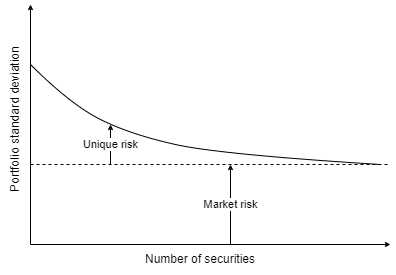
\includegraphics[width=0.57\textwidth,keepaspectratio]{risks}
\end{figure}
\begin{itemize}
    \item Risque unique / spécifique : risque pouvant être éliminé par la diversification
    \item Mais on ne peut pas éliminer tous les risques (ex : risque de marché / systématique)
\end{itemize}

\section{Résumé}

\begin{itemize}
    \item Le risque peut être mesuré : mesure de la dispersion des résultats futures $\rightarrow$ écart-type
    \item La diversification réduit le risque, mais toujours exposé aux changements macroéconomiques qui affectent la plupart des actions
    \item La prime de risque rémunère uniquement les risques non diversifiables
\end{itemize}

\chapter{Choix de portefeuille optimal / Capital Asset Pricing Model (CAPM / MEDAF)}

\begin{enumerate}
    \item Les investisseurs doivent détenir un portefeuille diversifié
    \item La prime de risque doit être proportionnelle au risque de marché
    \item[$\rightarrow$] Quelle est la prime de risque attendue pour détenir des actions ?
\end{enumerate}

\section{Hypothèses}

\begin{enumerate}
    \item[\textblue{H1}]: Les returns suivent une loi normale
    \item[\textblue{H2}]: Pas de coûts de transaction, pas de taxes et l'investisseur peut détenir n'importe quelle quantité de titres
    \item[\textblue{H3}]: L'information circule librement et est accessible gratuitement à tous les investisseurs
    \begin{itemize}
        \item Titres parfaitement identifiés par leur espérance $E[R_i]$, leur risque $\sigma [R_i]$ et leur corrélation avec tous les autres titres $\rho [R_i;R_j]$
        \item Tous les investisseurs positionnent les titres dans le même espace rentabilité - risque ($\sigma [R_i], E[R_i]$) $\rightarrow$ portefeuille optimal
    \end{itemize}
    \item[\textblue{H4}]: Les investisseurs maximisent leur rendement attendu pour un niveau de risque acceptable
    \item[\textblue{H5}]: Il est possible d'emprunter et de prêter au taux sans risque
\end{enumerate}

\section{Allocation optimale}

\subsection{Allocation entre un actif sans risque et un actif risqué}

\begin{itemize}
    \item Exprimer l'espérance de return en fonction du risque :
    \begin{align*}
               E[R_p] &= w_f r_f + w_1 E[R_1] \\
        \sigma^2[R_p] &= w_f^2 \sigma_f^2 + w_1^2 \sigma_1^2 + 2 w_f w_1 \rho{f1} \sigma_f \sigma1 \\
                      &= w_1^2 \sigma_1^2 \\
          \sigma[R_p] &= w_1 \sigma_1 \\
                      &\Downarrow \\
               E[R_p] &= R_f + \left( \frac{E[R_p] - R_f}{\sigma_1} \right) \sigma_p
    \end{align*}
    \item[$\rightarrow$] Le rendement du portefeuille est une fonction linéaire du risque
    \item[$\rightarrow$] $\sigma_{ptf}^2$ = Variance = Risque
\end{itemize}

\subsection{Allocation entre deux actifs risqués}

\begin{itemize}
    \item La rentabilité attendue et le risque sont données par :
    \begin{align*}
               E[R_p] &= w_1 E[R_1] + w_2 E[R_2] \\
        \sigma^2[R_p] &= w_1^2 \sigma_1^2 + w_2^2 \sigma_2^2 + 2 w_1 w_2 \rho{12} \sigma_1 \sigma2 \\
                    1 &= w_1 + w_2
    \end{align*}
    \item[$\rightarrow$] Modification de la forme de la frontière efficiente du portefeuille
\end{itemize}

\subsection{Allocation optimale entre N actifs risqués et un actif sans risque}

\textblue{Markowitz}
\begin{itemize}
    \item Les investisseurs maximisent leur espérance de rendement pour un risque acceptable
    \item Possibilité d'emprunter et de placer aux taux sans risques : portefeuille en partie dans le placement sans risque et dans le portefeuille $M$
    \item Les investisseurs qui veulent prendre plus de risque vont créer un effet levier en empruntant aux taux sans risque pour acheter le portefeuille $M$
    \item Le niveau de risque dépend uniquement du choix d'allocation entre $M$ et le taux sans risque $R_F$
\end{itemize}

\begin{figure}[H]
    \centering
    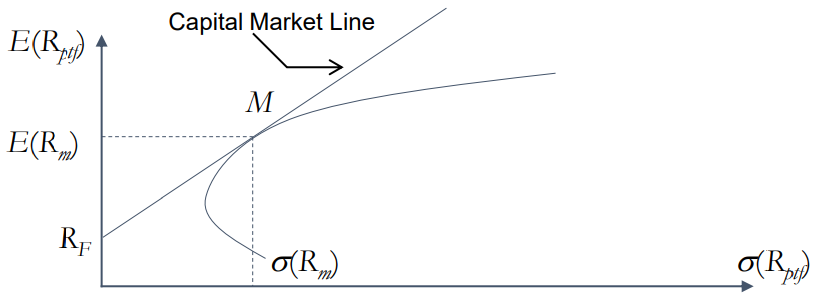
\includegraphics[width=0.57\textwidth,keepaspectratio]{markowitz}
\end{figure}
\begin{align*}
    E[R_ptf] &= R_f + \textgreen{\frac{E[R_m] - R_F}{\sigma_m} * \sigma_{ptf}}\\
    \frac{E[R_ptf] - R_F}{\sigma_{ptf}} &= \frac{E[R_m] - R_F}{\sigma_m}
\end{align*}
\begin{itemize}
    \item La \textgreen{prime de risque} est identique pour tous les portefeuilles optimaux
    \item Tous les portefeuilles situés sur la CML offrent la meilleure combinaison rendement-risque possible
\end{itemize}

\section{Portefeuille optimal et indice de marché}

\begin{itemize}
    \item Tous les investisseurs ont la même information, ils choisissent un portefeuille sur la Capital Market Line (CML)
    \item En fonction du niveau de risque acceptable, ils allouent :
    \begin{itemize}
        \item une partie au taux sans risque $w_f$
        \item une partie au portefeuille de marché $w_M$
    \end{itemize}
    \item Après allocation :
    \begin{itemize}
        \item prix des actions (et rendements attendus) à l'équilibre
        \item Tous les investisseurs détiennent le même portefeuille d'actifs risqués
        \item Les pondérations sont égales à la capitalisation boursière relative de chaque action $\rightarrow$ les indices sont des portefeuilles optimaux
    \end{itemize}
\end{itemize}

\section{Capital Asset Pricing Module (CAPM)}

\begin{itemize}
    \item Modèle d'équilibre des actifs financiers qui permet de déterminer la rentabilité attendue d'un actif en fonction de son risque systématique
    \item Permet d'estimer le rendement d'un actif en fonction de son risque :
    \begin{align*}
        E[R_i] &= R_f + \frac{E[R_m] - R_f}{\sigma_m} * \rho_{iM} \sigma_i \\
               &= R_f + \beta_i (E[R_m] - R_f)
    \end{align*}
    Où :
    \begin{align*}
    \beta_i &= \frac{\sigma(R_i, R_M)}{\sigma(R_M)} \\
            &= \frac{\rho_{iM} \sigma_i \sigma_M}{\sigma^2_M} \\
            &= \frac{\rho_{iM} \sigma_i}{\sigma_M}
    \end{align*}
    \begin{itemize}
        \item $\beta = 1$ : actif évolue en ligne avec le marché
        \item $\beta > 1$ : actif plus risqué que le marché
        \item $\beta < 1$ : actif moins risqué que le marché
    \end{itemize}
\end{itemize}

\section{Capital budgeting et WACC}

\begin{itemize}
    \item Coût marginal (ou coût d'opportunité du capital) est utilisé dans l'estimation du VAN d'un projet d'investissement
    \item Coût du capital = coût moyen pondéré de la dette et des fonds propres
    \item Coût de la dette ($E[R_D]$ = rendement de la dette et $\tau$ = taux d'imposition) :
    \begin{align*}
        K_D &= E[R_D] * (1 - \tau) \\
        E[R_m] &= YTM(\text{gvt}) + \text{spread}
    \end{align*}
    \item Coût des fonds propres :
    \begin{align*}
        K_E &= E[R_E] \\
        E[R_E] &= R_f + \beta * (E[R_M] - R_f)
    \end{align*}
    \item Coût moyen pondéré du capital (WACC)
    \begin{align*}
        WACC = \frac{D}{D + E} * K_D + \frac{E}{D + E} * K_E
    \end{align*}
\end{itemize}

\section{Questions}

\subsection{Quel est le portefeuille optimal ?}

\begin{itemize}
    \item Diversifié : risques spécifiques éliminés par diversification, seul le risque systématique subsiste
    \item Composé d'un placement sans risque et d'un investissement dans le portefeuille marché
    \item Pour modifier le risque du portefeuille, il faut modifier l'allocation
\end{itemize}

\subsection{Quelle est la rentabilité attendue d'un portefeuille optimal ?}

\begin{align*}
    E[R_p] = R_f + \frac{E[R_M] - R_F}{\sigma_M} * \sigma_P
\end{align*}
\begin{itemize}
    \item La prime de risque est proportionnelle au risque total (systématique)
\end{itemize}

\subsection{Quelle est la rentabilité attendue d'un actif risqué ?}

\begin{itemize}
    \item Pas le risque du titre qui est essentiel, mais la contribution du titre au risque du portefeuille de marché
\end{itemize}
\begin{align*}
    E[R_i] = R_f \frac{E[R_M] - R_f}{\sigma_M} * \rho_{iM} * \sigma_i
\end{align*}

\subsection{Quelle est l'allocation optimale au sein du portefeuille marché ?}

Le poids des titres ($w_1, \ldots, w_N$) dans le portefeuille optimal sont proportionnels aux capitalisations boursières relatives des titres.

\addtocounter{chapter}{2}
\chapter{Structure financière dans un marché parfait}

\section{Sans taxation, la valeur d'une entreprise dépend-elle de la structure financière ?}

\begin{itemize}
    \item \textblue{Modigliani and Miller} (1958) : Lorsqu'il n'y a pas d'impôts et que le \textgreen{marché des capitaux fonctionnent bien}, la valeur de marché d'une entreprise ne dépend pas de la structure de son capital
    \begin{itemize}
        \item[\textgreen{$\rightarrow$}] Les investisseurs peuvent négocier des titres sans restriction et peuvent emprunter et prêter aux mêmes conditions que l'entreprise
        \item[\textgreen{$\rightarrow$}] Pas d'impôts ni de coûts de détresse financière
    \end{itemize}
    \item \textblue{Différence entre le ROI et le ROE} :\\
    Soit deux entreprises, une avec que des fonds propres et l'autre avec une dette en plus
    \begin{itemize}
        \item \textblue{ROI} : reste le même dans les deux cas : $\frac{EBIT}{\# \text{ d'actifs}}$
        \item \textblue{ROE} : permet un effet levier : $KOI + \frac{D}{E} (ROE - T_d)$ où
        \begin{itemize}
            \item $E$ = Fonds propres
            \item $D$ = Dette
            \item $\frac{D}{E}$ = Ratio d'endettement
            \item $I_d$ = share price / taux d'intérêt sur la dette
        \end{itemize}
        \item ROE > ROI est mauvais signe
    \end{itemize}
\end{itemize}

\section{Endettement et relation rentabilité-risque}

\begin{itemize}
    \item Le financement par emprunt n'affecte pas le \textgreen{risque d'exploitatio}n (risque commercial) mais il ajoute un risque financier
    \item[\textgreen{$\rightarrow$}] Lié aux opérations courantes de l'entreprise (ventes, coût de production, gestion des stocks) $\rightarrow$ n'influence pas la demande du marché, la concurrence ni les coûts variables
    \item Le risque financier est lié à l'obligation de rembourser les intérêts et le principal de la dette
    \begin{itemize}
        \item + sensible aux variations de revenus. Si le revenu diminue, l'entreprise peut avoir du mal à couvrir ses obligations de dettes (augmentation du risque de défaut)
        \item Si l'entreprise emprunte pour racheter la moitié de ses actions, alors la même quantité de risque opérationnel est supportée par la moitié de fonds propres, le risque par action doit doubler
        \item L'effet levier augmente le bénéfice attendu par action, mais il augmente également le risque, et ainsi le taux d'actualisation
    \end{itemize}
\end{itemize}

\subsection{Endettement et coût des fonds propres}

\begin{itemize}
    \item Comme la restructuration ne modifie ni le résultat d'exploitation ni la valeur de l'entreprise, elle ne modifie pas non plus le coût du capital (pas d'impôts !)
    \begin{align*}
        WACC = r_{\text{assets}} = \frac{D}{D + E} * r_{\text{debt}} + \frac{E}{D + E} * r_{\text{equity}}
    \end{align*}
    \item Modigliani Miller (2) : le taux de rendement attendu des actions d'une entreprise à effet de levier augmente proportionnellement au ratio dette / fonds propres exprimé en valeur de marché
    \begin{align*}
        r_{\text{equity}} = r_{\text{asset}} + \frac{D}{E} * (r_{\text{asset}} - r_{\text{debt}})
    \end{align*}
    \item EBT = Earnings Before Tax
    \item EAT = Earnings After Tax
    \item Coût du capital :
    \begin{align*}
        WACC = \frac{D}{D + E} * r_{\text{debt}} * (1 - \tau) + \frac{E}{D + E} * r_{\text{equity}}
    \end{align*}
\end{itemize}

\begin{figure}[H]
    \centering
    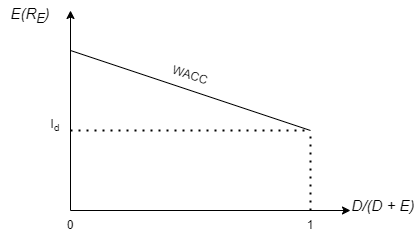
\includegraphics[width=0.57\textwidth,keepaspectratio]{wacc}
\end{figure}
\begin{itemize}
    \item En $0$ : intro de la dette
    \item En $1$ : le ratio $\frac{D}{E}$ augmente $\rightarrow$ augmente le risque financier $\rightarrow$ augmente le coût des capitaux propres
    \item[$\rightarrow$] Effet levier $> 0$ : introduire un certain niveau de dette $\rightarrow$ diminution du $WACC$ car la dette est moins couteuse que les capitaux propres
    \item[$\rightarrow$] Effet de risque financier : au-delà d'un certain niveau d'endettement, augmentation du risque financier $\rightarrow$ augmentation du coût des capitaux propres $\rightarrow$ augmentation du $WACC$
\end{itemize}

\subsection{Limite de l'économie fiscale}

Pour bénéficier des avantages fiscaux de la dette, une entreprise doit avoir des bénéfices imposables
\begin{itemize}
    \item Avantages fiscaux : les intérêts payés sur la dette sont généralement déductibles des impôts $\rightarrow$ diminue le résultat imposable et donc diminue les impôts
    \item utilisation de la dette pour diminuer la charge fiscale et augmentation de la rentabilité nette
\end{itemize}

\subsection{Niveau de dette maximum}

Pour éviter les intérêts inaccessibles, une entreprise dont les bénéfices sont positifs doit avoir un niveau d'endettement t.q. les paiements d'intérêts sont inférieurs à ses bénéfices imposables prévus
\begin{align*}
    Interest = r_D * \text{Debt} \leq EBIT
\end{align*}

\subsection{Coût de détresse financière}

\begin{itemize}
    \item Coûts supplémentaires auxquels une entreprise soit faite lorsqu'elle est fortement endettée et qu'elle approuve des difficultés à honorer ses engagements financiers
    \item Déclenchement :
    \begin{itemize}
        \item Accroissement de la prime de risque (spread) pour compenser le risque lié au remboursement de la dette
        \item Restructuration forcée (coûts juridiques et financiers)
        \item Défaut ou faillite
    \end{itemize}
    \item Théorie du compromis (trade-off theory) : la valeur de l'entreprise endettée est le résultat d'un compromis entre les avantages fiscaux liés à la dette et les coûts de détresse financière liés à un endettement abusif
    \begin{itemize}
        \item Valeur de la firme endettée = valeur de la firme non endettée + valeur actuelle de l'économie fiscale - valeur actuelle des coûts de détresse financière
    \end{itemize}
\end{itemize}
